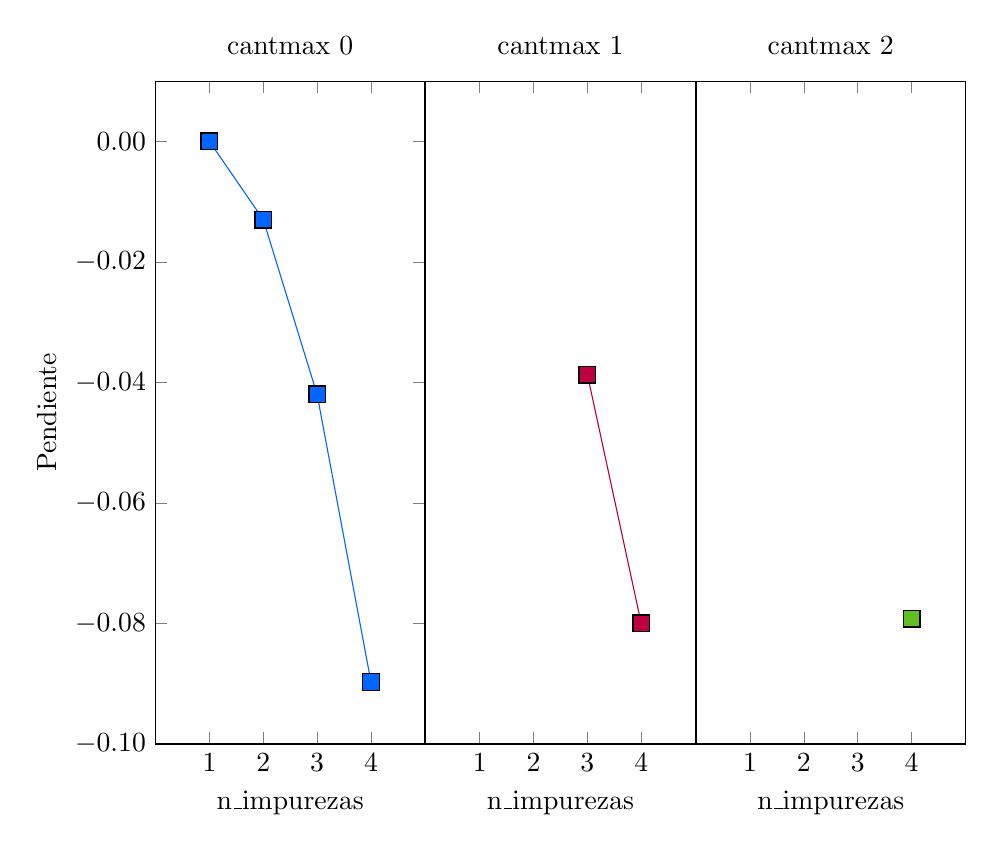
\begin{tikzpicture}[scale=1]
    % Primer gráfico
    \begin{axis}[
        title= cantmax 0,
        width=5cm,
        height=10cm,
        name=plot1,
        xlabel= n\_impurezas ,
        ylabel={Pendiente},
        xmin=0, xmax=5,
        ymin=-0.1, ymax=0.01,
        yticklabel style={
            /pgf/number format/.cd,
            fixed,
            fixed zerofill,
            precision=2,
            /tikz/.cd
        },
        scaled y ticks=false,
        xtick=data,
    ]
    \addplot[blue!60!cyan, mark=square*, mark size = 3pt, mark options={draw=black,line width = 0.5pt}] coordinates {(1,0) (2,-0.013) (3,-0.042) (4,-0.0897)};
    %\node[left] at (axis cs:1,0) {0};
    %\node[left] at (axis cs:2,-0.013) {-0.013};
    %\node[left] at (axis cs:3,-0.042) {-0.042};
    %\node[left] at (axis cs:4,-0.0897) {-0.0897};
    \end{axis}
    
    % Segundo gráfico
    \begin{axis}[
        title= cantmax 1,
        width=5cm,
        height=10cm,
        name=plot2,
        at={(plot1.outer east)},
        anchor=outer west,
        %xshift=1cm, % Distancia entre gráficos
        xlabel= n\_impurezas ,
        xmin=0, xmax=5,
        ymin=-0.1, ymax=0.01,
        yticklabel style={
            /pgf/number format/.cd,
            fixed,
            fixed zerofill,
            precision=2,
            /tikz/.cd
        },
        scaled y ticks=false,
        ytick=\empty, % Elimina las marcas del eje y
        ylabel={}, % Elimina la etiqueta del eje y
        legend style={at={(0.5,-0.2)},anchor=north},
        %mostramos todas las xticks 1, 2, 3 ,4
        xtick={1,...,4}
    ]
    \addplot[purple, mark=square*, mark size = 3pt, mark options={draw=black,line width = 0.5pt}] coordinates {(3,-0.0387) (4,-0.08)};
    %\node[left] at (axis cs:2,-0.0387) {-0.0387};
    %\node[left] at (axis cs:3,-0.08) {-0.08};
    
    \end{axis}
    
    % Tercer gráfico
    \begin{axis}[
        title= cantmax 2,
        width=5cm,
        height=10cm,
        at={(plot2.outer east)},
        anchor=outer west,
        %xshift=2cm,
        xlabel= n\_impurezas ,
        xmin=0, xmax=5,
        ymin=-0.1, ymax=0.01,
        yticklabel style={
            /pgf/number format/.cd,
            fixed,
            fixed zerofill,
            precision=2,
            /tikz/.cd
        },
        scaled y ticks=false,
        ytick=\empty, % Elimina las marcas del eje y
        ylabel={}, % Elimina la etiqueta del eje y
        legend style={at={(0.5,-0.2)},anchor=north},
        xtick={1,...,4}
    ]
    \addplot[green!50!brown, mark=square*, mark size = 3pt, mark options={draw=black,line width = 0.5pt}] coordinates { (4,-0.0792)};
    %\node[left] at (axis cs:4,-0.0792) {-0.0792};
    
    \end{axis}
\end{tikzpicture}